%% bare_jrnl.tex
%% V1.3
%% 2007/01/11
%% by Michael Shell
%% see http://www.michaelshell.org/
%% for current contact information.
%%
%% This is a skeleton file demonstrating the use of IEEEtran.cls
%% (requires IEEEtran.cls version 1.7 or later) with an IEEE journal paper.
%%
%% Support sites:
%% http://www.michaelshell.org/tex/ieeetran/
%% http://www.ctan.org/tex-archive/macros/latex/contrib/IEEEtran/
%% and
%% http://www.ieee.org/

% This file has been modified for use in the ECE 111 course offered at OSU. This includes
% renaming files, modifying current text, and removing large portions of the .tex file to reduce student confusion.
%
% Modifier's contact information
% Matthew Shuman
% ECE 111 Instructor at Oregon State University

%%*************************************************************************
%% Legal Notice:
%% This code is offered as-is without any warranty either expressed or
%% implied; without even the implied warranty of MERCHANTABILITY or
%% FITNESS FOR A PARTICULAR PURPOSE! 
%% User assumes all risk.
%% In no event shall IEEE or any contributor to this code be liable for
%% any damages or losses, including, but not limited to, incidental,
%% consequential, or any other damages, resulting from the use or misuse
%% of any information contained here.
%%
%% All comments are the opinions of their respective authors and are not
%% necessarily endorsed by the IEEE.
%%
%% This work is distributed under the LaTeX Project Public License (LPPL)
%% ( http://www.latex-project.org/ ) version 1.3, and may be freely used,
%% distributed and modified. A copy of the LPPL, version 1.3, is included
%% in the base LaTeX documentation of all distributions of LaTeX released
%% 2003/12/01 or later.
%% Retain all contribution notices and credits.
%% ** Modified files should be clearly indicated as such, including  **
%% ** renaming them and changing author support contact information. **
\documentclass[journal]{IEEEtran}

% *** GRAPHICS RELATED PACKAGES ***
%
\ifCLASSINFOpdf
   \usepackage[pdftex]{graphicx}
  % declare the path(s) where your graphic files are
   \graphicspath{{../pdf/}{../jpeg/}}
  % and their extensions so you won't have to specify these with
  % every instance of \includegraphics
   \DeclareGraphicsExtensions{.pdf,.jpeg,.png}
\else
   \usepackage[dvips]{graphicx}
  % declare the path(s) where your graphic files are
   \graphicspath{{../eps/}}
  % and their extensions so you won't have to specify these with
  % every instance of \includegraphics
   \DeclareGraphicsExtensions{.eps}
\fi

\begin{document}
%
% paper title
% can use linebreaks \\ within to get better formatting as desired
\title{ECE 111 Final Report}

\author{Student~Name,~ECE 111 Student
\thanks{Thanks to M. Shell with the Department
of Electrical and Computer Engineering, Georgia Institute of Technology, Atlanta,
GA, 30332 USA e-mail: (see http://www.michaelshell.org/contact.html) for providing this template.}% <-this % stops a space
\thanks{M. Shuman for modifying the template for use in ECE 111 at Oregon State University.}}

% The paper headers
\markboth{ECE 111 \LaTeX\ Report,~No.~1, Fall~2017}%
{Shell \MakeLowercase{\textit{et al.}}:ECE 111 Final Report}

% make the title area
\maketitle

\begin{abstract}
%\boldmath
The abstract goes here.  Use this paragraph to summarize your experience with ECE 111.  Include a brief summary of the portions of the course and the overall goal of the course.
\end{abstract}

% Note that keywords are not normally used for peerreview papers.
\begin{IEEEkeywords}
IEEEtran, journal, \LaTeX, paper, template.
\end{IEEEkeywords}

\section{Introduction}
% The very first letter is a 2 line initial drop letter followed
% by the rest of the first word in caps.
% 
% form to use if the first word consists of a single letter:
% \IEEEPARstart{A}{demo} file is ....
% 
% form to use if you need the single drop letter followed by
% normal text (unknown if ever used by IEEE):
% \IEEEPARstart{A}{}demo file is ....
% 
% Some journals put the first two words in caps:
% \IEEEPARstart{T}{his demo} file is ....
% 
% Here we have the typical use of a "T" for an initial drop letter
% and "HIS" in caps to complete the first word.
\IEEEPARstart{T}{his} demo file is intended to serve as a ``starter file''
for the ECE 111 final report produced under \LaTeX\ using
IEEEtran.cls version 1.7 and later.
% You must have at least 2 lines in the paragraph with the drop letter
% (should never be an issue)
I wish you the best of success in your pursuit of education at OSU and with opportunities after OSU.  Read "On Writing Well", by William Zinsser if you struggle with writing\cite{Zinsser1976}.  Read "On Writing Well", by William Zinsser if you don't struggle with writing and want to improve your abilities.

\hfill mws
 
\hfill November 8th, 2017

What is the required topic of the report?  You need to cover the following topics, and here is how you will cite one of your sources\cite{OSU2016}.

Students always ask "How long does the report needs to be?"  They really mean "How short can the report be and still get a decent grade?"  That's an interesting question.  The key indicator of report quality isn't length, but it's explaining the background and context of an idea, explaining the idea thoroughly, and then explaining how this idea links to the next idea.  

For example, don't simply state the cost of attendance at OSU.  Relate that cost to other universities.  Has the cost of OSU changed recently?  Is the cost going up or staying relatively constant?  What would you estimate the cost to be when you're a senior?  There are many factors to consider when evaluating something straightforward as cost of attendance.  Don't just state the cost is \$25,434/year\cite{OSU2016} (Note that the cost is \$26,046 in 2017).  Be thorough with your report.  It's worth 15\% of your final grade in ECE 111.  Use a variety of reliable sources...
\cite{HECC2015}\cite{DeptOfEdu2016}\cite{Gazette2012}\cite{OUS2013}\cite{TuitionHistory2017}.  Also, cite your source if you use information in your report (use information in your report).
%TL;DR (4-5 pages, IEEE format)

\section{Finances}
The following latin is a common space filler to show what the document will look like when text is inserted.

Lorem ipsum dolor sit amet, consectetur adipiscing elit. Ut libero mauris, porta tincidunt urna fringilla, tincidunt scelerisque lorem. Nunc sem mi, viverra quis turpis rhoncus, egestas lobortis neque. In hac habitasse platea dictumst. Sed a volutpat urna. Mauris aliquet orci vitae lorem feugiat, ut lobortis ipsum bibendum. Suspendisse tincidunt eget orci sed fermentum. Quisque non risus aliquam risus varius rutrum id et sapien.

Vestibulum porta fringilla ante, sed mattis elit mollis in. Morbi volutpat eros nec pulvinar efficitur. Praesent pharetra posuere nisi sit amet faucibus. Nam pretium odio tortor, eu faucibus turpis eleifend in. Vestibulum eu risus purus. Vestibulum bibendum justo a tempus facilisis. Proin id eleifend quam.

Nunc nec lectus sed mauris bibendum suscipit. Quisque eget tortor bibendum, aliquam felis bibendum, pulvinar leo. Cras accumsan et dolor vel sodales. Vestibulum tincidunt augue nec ipsum sagittis, eget placerat felis commodo. Suspendisse leo enim, euismod ut lectus at, sollicitudin fermentum sapien. Lorem ipsum dolor sit amet, consectetur adipiscing elit. Suspendisse pellentesque turpis vitae lorem accumsan pellentesque. Quisque auctor mi ac ex mattis, ac lacinia urna scelerisque. Fusce aliquet neque sem, eu aliquam diam feugiat porttitor. Sed sollicitudin elit ac dolor cursus hendrerit. Ut ultricies metus in sollicitudin consequat. Morbi dapibus elit at tempus cursus. Integer vel condimentum felis, sed porta tortor.
\subsection{Cost of attendance}
Lorem ipsum dolor sit amet, consectetur adipiscing elit. Ut libero mauris, porta tincidunt urna fringilla, tincidunt scelerisque lorem. Nunc sem mi, viverra quis turpis rhoncus, egestas lobortis neque. In hac habitasse platea dictumst. Sed a volutpat urna. Mauris aliquet orci vitae lorem feugiat, ut lobortis ipsum bibendum. Suspendisse tincidunt eget orci sed fermentum. Quisque non risus aliquam risus varius rutrum id et sapien.

\subsection{Minimizing costs}
Lorem ipsum dolor sit amet, consectetur adipiscing elit. Ut libero mauris, porta tincidunt urna fringilla, tincidunt scelerisque lorem. Nunc sem mi, viverra quis turpis rhoncus, egestas lobortis neque. In hac habitasse platea dictumst. Sed a volutpat urna. Mauris aliquet orci vitae lorem feugiat, ut lobortis ipsum bibendum. Suspendisse tincidunt eget orci sed fermentum. Quisque non risus aliquam risus varius rutrum id et sapien.

\subsection{Internship income}
Lorem ipsum dolor sit amet, consectetur adipiscing elit. Ut libero mauris, porta tincidunt urna fringilla, tincidunt scelerisque lorem. Nunc sem mi, viverra quis turpis rhoncus, egestas lobortis neque. In hac habitasse platea dictumst. Sed a volutpat urna. Mauris aliquet orci vitae lorem feugiat, ut lobortis ipsum bibendum. Suspendisse tincidunt eget orci sed fermentum. Quisque non risus aliquam risus varius rutrum id et sapien.

\subsection{Scholarships}
Lorem ipsum dolor sit amet, consectetur adipiscing elit. Ut libero mauris, porta tincidunt urna fringilla, tincidunt scelerisque lorem. Nunc sem mi, viverra quis turpis rhoncus, egestas lobortis neque. In hac habitasse platea dictumst. Sed a volutpat urna. Mauris aliquet orci vitae lorem feugiat, ut lobortis ipsum bibendum. Suspendisse tincidunt eget orci sed fermentum. Quisque non risus aliquam risus varius rutrum id et sapien.

\subsection{Loan types}
Lorem ipsum dolor sit amet, consectetur adipiscing elit. Ut libero mauris, porta tincidunt urna fringilla, tincidunt scelerisque lorem. Nunc sem mi, viverra quis turpis rhoncus, egestas lobortis neque. In hac habitasse platea dictumst. Sed a volutpat urna. Mauris aliquet orci vitae lorem feugiat, ut lobortis ipsum bibendum. Suspendisse tincidunt eget orci sed fermentum. Quisque non risus aliquam risus varius rutrum id et sapien.

\subsection{After graduation salary}
Lorem ipsum dolor sit amet, consectetur adipiscing elit. Ut libero mauris, porta tincidunt urna fringilla, tincidunt scelerisque lorem. Nunc sem mi, viverra quis turpis rhoncus, egestas lobortis neque. In hac habitasse platea dictumst. Sed a volutpat urna. Mauris aliquet orci vitae lorem feugiat, ut lobortis ipsum bibendum. Suspendisse tincidunt eget orci sed fermentum. Quisque non risus aliquam risus varius rutrum id et sapien.

\section{Textbook}
\subsection{Chapter 1}
\subsection{Chapter 2}
\subsection{Chapter 3}
\subsection{Chapter 4}
\subsection{Chapter 5}
\subsection{Chapter 6}
\subsection{Chapter 7}

\section{Lab}
\subsection{Hardware}
\subsection{Software}
\subsubsection{LaTex}
\subsubsection{C++}
\subsubsection{Python}
\subsection{Activities}
\subsubsection{Lab 1}
\subsubsection{Lab 2}
\subsubsection{Lab 3}
\subsubsection{Lab 4}
\subsubsection{Lab 5}
\subsubsection{Lab 6}

\section{Guest Speakers}
These speakers can be from the ECE 111 lecture, or you may listen to a TED talk and use that information to help guide your future plans with ECE.
\subsection{1st Speaker}
\subsection{2nd Speaker}


% An example of a floating figure using the graphicx package.
% Note that \label must occur AFTER (or within) \caption.
% For figures, \caption should occur after the \includegraphics.
% Note that IEEEtran v1.7 and later has special internal code that
% is designed to preserve the operation of \label within \caption
% even when the captionsoff option is in effect. However, because
% of issues like this, it may be the safest practice to put all your
% \label just after \caption rather than within \caption{}.
%
%
\begin{figure}[!t]
\centering
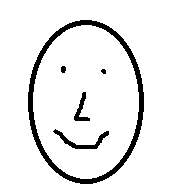
\includegraphics[width=2.5in]{face.png}
% where an .eps filename suffix will be assumed under latex, 
 %and a .pdf suffix will be assumed for pdflatex; or what has been declared
 %via \DeclareGraphicsExtensions.
\caption{Here's an example image}
\label{fig:example}
\end{figure}

% Note that IEEE typically puts floats only at the top, even when this
% results in a large percentage of a column being occupied by floats.


\section{Conclusion}
The conclusion goes here. Use this section to tie all of the experiences within ECE 111 together.  ECE 111 has three fundamental questions.  
\begin{enumerate}
\item Do you really know what ECE entails?  
\item Is ECE the right major for you?
\item Are you willing to work hard and learn the necessary skills?
\end{enumerate}
This refers to the number of the figure with a reference to Figure \ref{fig:example}.

% use appendices with more than one appendix
% then use \section to start each appendix
% you must declare a \section before using any
% \subsection or using \label (\appendices by itself
% starts a section numbered zero.)
%
\appendices
\section{Proof of the First Zonklar Equation}
The ECE 111 Report probably doesn't need an appendix, but here's how one could add an appendix.

% you can choose not to have a title for an appendix
% if you want by leaving the argument blank
\section{}
Appendix two text goes here.


% use section* for acknowledgement
\section*{Acknowledgment}


I would like to thank ...


%\bibliography{IEEEabrv,../bib/paper}
\bibliography{Biblio.bib}
\bibliographystyle{IEEEtran} 

% biography section
% 
% If you have an EPS/PDF photo (graphicx package needed) extra braces are
% needed around the contents of the optional argument to biography to prevent
% the LaTeX parser from getting confused when it sees the complicated
% \includegraphics command within an optional argument. (You could create
% your own custom macro containing the \includegraphics command to make things
% simpler here.)
:

\begin{biography}[{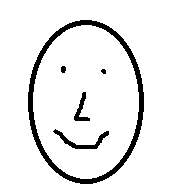
\includegraphics[width=1in,height=1.25in,clip,keepaspectratio]{face.png}}]{John Doe}
Biography text here.
\end{biography}

% if you will not have a photo at all:
\begin{IEEEbiographynophoto}{Matthew Shuman}
Matthew Shuman received his Masters in ECE in September 2008 from Oregon State University.  He has since become an instructor for many ECE courses offered at OSU.
\end{IEEEbiographynophoto}

% insert where needed to balance the two columns on the last page with
% biographies
%\newpage

\begin{IEEEbiographynophoto}{Jane Doe}
Biography text here.  Use this information to list some of your background relating to ECE, OSU, or other relevant background information.
\end{IEEEbiographynophoto}

% You can push biographies down or up by placing
% a \vfill before or after them. The appropriate
% use of \vfill depends on what kind of text is
% on the last page and whether or not the columns
% are being equalized.

%\vfill

% Can be used to pull up biographies so that the bottom of the last one
% is flush with the other column.
%\enlargethispage{-5in}



% that's all folks
\end{document}


